% *********************************************************************
% © 2016–2019 Jeremy Sylvestre
%
% Permission is granted to copy, distribute and/or modify this document
% under the terms of the GNU Free Documentation License, Version 1.3 or
% any later version published by the Free Software Foundation; with no
% Invariant Sections, no Front-Cover Texts, and no Back-Cover Texts. A
% copy of the license is included in the appendix entitled “GNU Free
% Documentation License” that appears in the output document of this
% PreTeXt source code. All trademarks™ are the registered® marks of
% their respective owners.
% 
% *********************************************************************
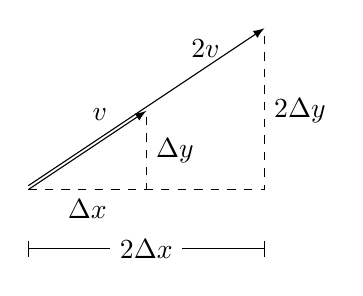
\begin{tikzpicture}[
	point/.style={circle,draw,very thin,fill,inner sep=0pt,minimum size=4pt},
	vector/.style={-latex},
]
	\draw[vector] (0,0) to node[above left,near end] {$\uvec{v}$} (1.5,1);
	\draw[vector] (0,0.05) to node[above,near end] {$2\uvec{v}$} (3,2.05);
	\draw[dashed] (0,0) to node[below] {$\Delta x$} (1.5,0) to node[right] {$\Delta y$} (1.5,1);
	\draw[dashed] (0,0) to (3,0) to node[right] {$2\Delta y$} (3,2);
	\node (ddx) at (1.5,-0.75) {$2\Delta x$};
	\draw (0,-0.75) to (ddx.west);
	\draw (ddx.east) to (3,-0.75);
	\draw (0,-0.65) to (0,-0.85);
	\draw (3,-0.65) to (3,-0.85);
\end{tikzpicture}
